\documentclass{assignment}
\usepackage{float}
\usepackage{lipsum}
\usepackage[document]{ragged2e}
\usepackage{tcolorbox}
\usepackage{array}
\usepackage{geometry}
\usepackage{xcolor}
\usepackage{booktabs}
\usepackage{caption}
\usepackage[table]{xcolor}

\geometry{a4paper, margin=1in}

\definecolor{lightblue}{RGB}{37, 150, 190}

\newtcolorbox{exercisebox}{
  colback=lightblue!10,
  colframe=lightblue,
  arc=5pt,
  boxrule=1pt,
  boxsep=10pt,
  left=15pt,
  right=15pt,
  top=10pt,
  bottom=10pt,
  center,
}

\begin{document}
\assignmentTitle{Padova (PD)}{17 Ottobre 2024}{assets/logoAR.png}{Design Network Aziendale}{IT Support and Cybersecurity}

\section{Caratteristiche di Progetto}

\begin{center}
\begin{exercisebox}
\subsection{Caratteristiche del Nuovo Ufficio}

L'ufficio avrà le seguenti caratteristiche:

\begin{itemize}
    \item \textbf{Numero di persone}: 30
    \item \textbf{Sistemi operativi}: Mac e Windows
    \item \textbf{Superficie}: 300 metri quadri
    \item \textbf{Posizione}: Centro storico di una piccola cittadina (meno di 50.000 abitanti)
\end{itemize}

\subsection{Distribuzione degli Ambienti}

L'ufficio sarà suddiviso in 8 ambienti utilizzati come segue:

\begin{enumerate}
    \item \textbf{Ufficio 1}: 1 computer
    \item \textbf{Ufficio 2}: 10 computer
    \item \textbf{Ufficio 3}: 10 computer
    \item \textbf{Ufficio 4}: Sala relax
    \item \textbf{Ufficio 5}: Sala stampante / magazzino
    \item \textbf{Ufficio 6}: 5 computer
    \item \textbf{Ufficio 7}: Sala meeting con sistema di videoconferenza
    \item \textbf{Ufficio 8}: Sala rete
\end{enumerate}
\end{exercisebox}
\end{center}

\section*{Obiettivi Progettuali}

Il progetto per la nuova infrastruttura di rete ha diversi obiettivi chiave, volti a garantire che la rete offra prestazioni elevate, sicurezza e scalabilità per supportare l'espansione futura dell'azienda. Di seguito, riassumiamo gli obiettivi principali:

\begin{table}[H]
\centering
\begin{tabular}{|>{\bfseries}m{4cm}|m{8cm}|m{5cm}|}    
    \toprule
    \rowcolor{lightblue} Obiettivo & Descrizione \\
    \midrule
    Prestazioni elevate & Garantire una rete rapida e affidabile per supportare tutti i dipendenti \\
    \midrule
    Sicurezza & Implementare misure avanzate di protezione, come firewall e crittografia \\
    \midrule
    Scalabilità & Progettare la rete per permettere future espansioni senza interventi invasivi \\
    \midrule
    Affidabilità & Ridurre i tempi di inattività con ridondanza e monitoraggio continuo \\
    \midrule
    Facilità di gestione & Utilizzare strumenti di monitoraggio e gestione per semplificare la manutenzione \\
    \bottomrule
\end{tabular}
\caption{Riassunto degli obiettivi progettuali}
\end{table}

\section{Location Ufficio}

L'ufficio si trova nel centro storico di Scandicci, una piccola cittadina con circa 50.000 abitanti. Questa posizione richiede una connessione Internet affidabile e veloce, in quanto è presente un numero elevato di clienti e fornitori che richiedono comunicazioni regolari.


L'indirizzo dell'ufficio è:

\begin{exercisebox}
    \begin{center}
        \textbf{Piazzale della Resistenza 8, 50018 Scandicci (FI)}.
    \end{center}
\end{exercisebox}



\section{Scelta degli Operatori e Connettività}
La connettività scelta è la \textbf{FTTH} poiché garantisce la massima velocità e bassa latenza, ideale per gestire videoconferenze e carichi di lavoro elevati. Inoltre, fornisce una maggiore stabilità rispetto alle alternative come \textbf{FTTC} (Fiber to the Cabinet) o connessioni wireless.

Dopo aver effettuato una ricerca, propongo due operatori per l'accesso a Internet presso l'ufficio:

\begin{enumerate}
    \item \textbf{TIM Business}: offre una connessione in fibra ottica \textbf{FTTH} (Fiber to the Home) con velocità fino a 2.5 Gbps in download e 300 Mbps in upload. Costo mensile: 24,90 €.
    \item \textbf{Fastweb Business}: offre una connessione in fibra ottica con velocità fino a 1 Gbps in download e 300 Mbps in upload. Costo mensile: da 31,95 €.
\end{enumerate}


\begin{table}[H]
    \centering
    \begin{tabular}{|>{\bfseries}m{4cm}|m{5cm}|m{5cm}|}
        \toprule
        \rowcolor{lightblue} 
        \textbf{Caratteristica} & \textbf{TIM Business - Full Fibra} & \textbf{Fastweb Business} \\
        \midrule
        Velocità Fibra & Fino a 2.5 Gbps & Fino a 1Gb \\
        \midrule
        Chiamate & Illimitate verso fissi e mobili & Illimitate \\
        \midrule
        IP Statico & Incluso & Non specificato \\
        \midrule
        Router & Wi-Fi 6 (opzionale) & Internet Box NeXXt One incluso \\
        \midrule
        Assistenza & Assistenza Tecnica a 360° & Assicurazione ai locali commerciali con Quixa \\
        \midrule
        Corsi Digitali & Non disponibile & Fastweb Digital Academy inclusa \\
        \midrule
        Prezzo & 24,90 \texteuro/mese (dopo 3 mesi di promozione) & Da 31,95 \texteuro/mese \\
        \bottomrule
    \end{tabular}
    \caption{Confronto tra le offerte TIM Business e Fastweb Business}
    \end{table}

Abbiamo scelto di utilizzare TIM come connessione principale e Fastware come connessione di backup, così da avere una ridondanza della connessione e poter garantire la continuità del servizio in caso di guasti o interruzioni di uno dei due operatori.

\section{Planimetria dell'Ufficio}

La planimetria dell'ufficio è la seguente:

\begin{center}
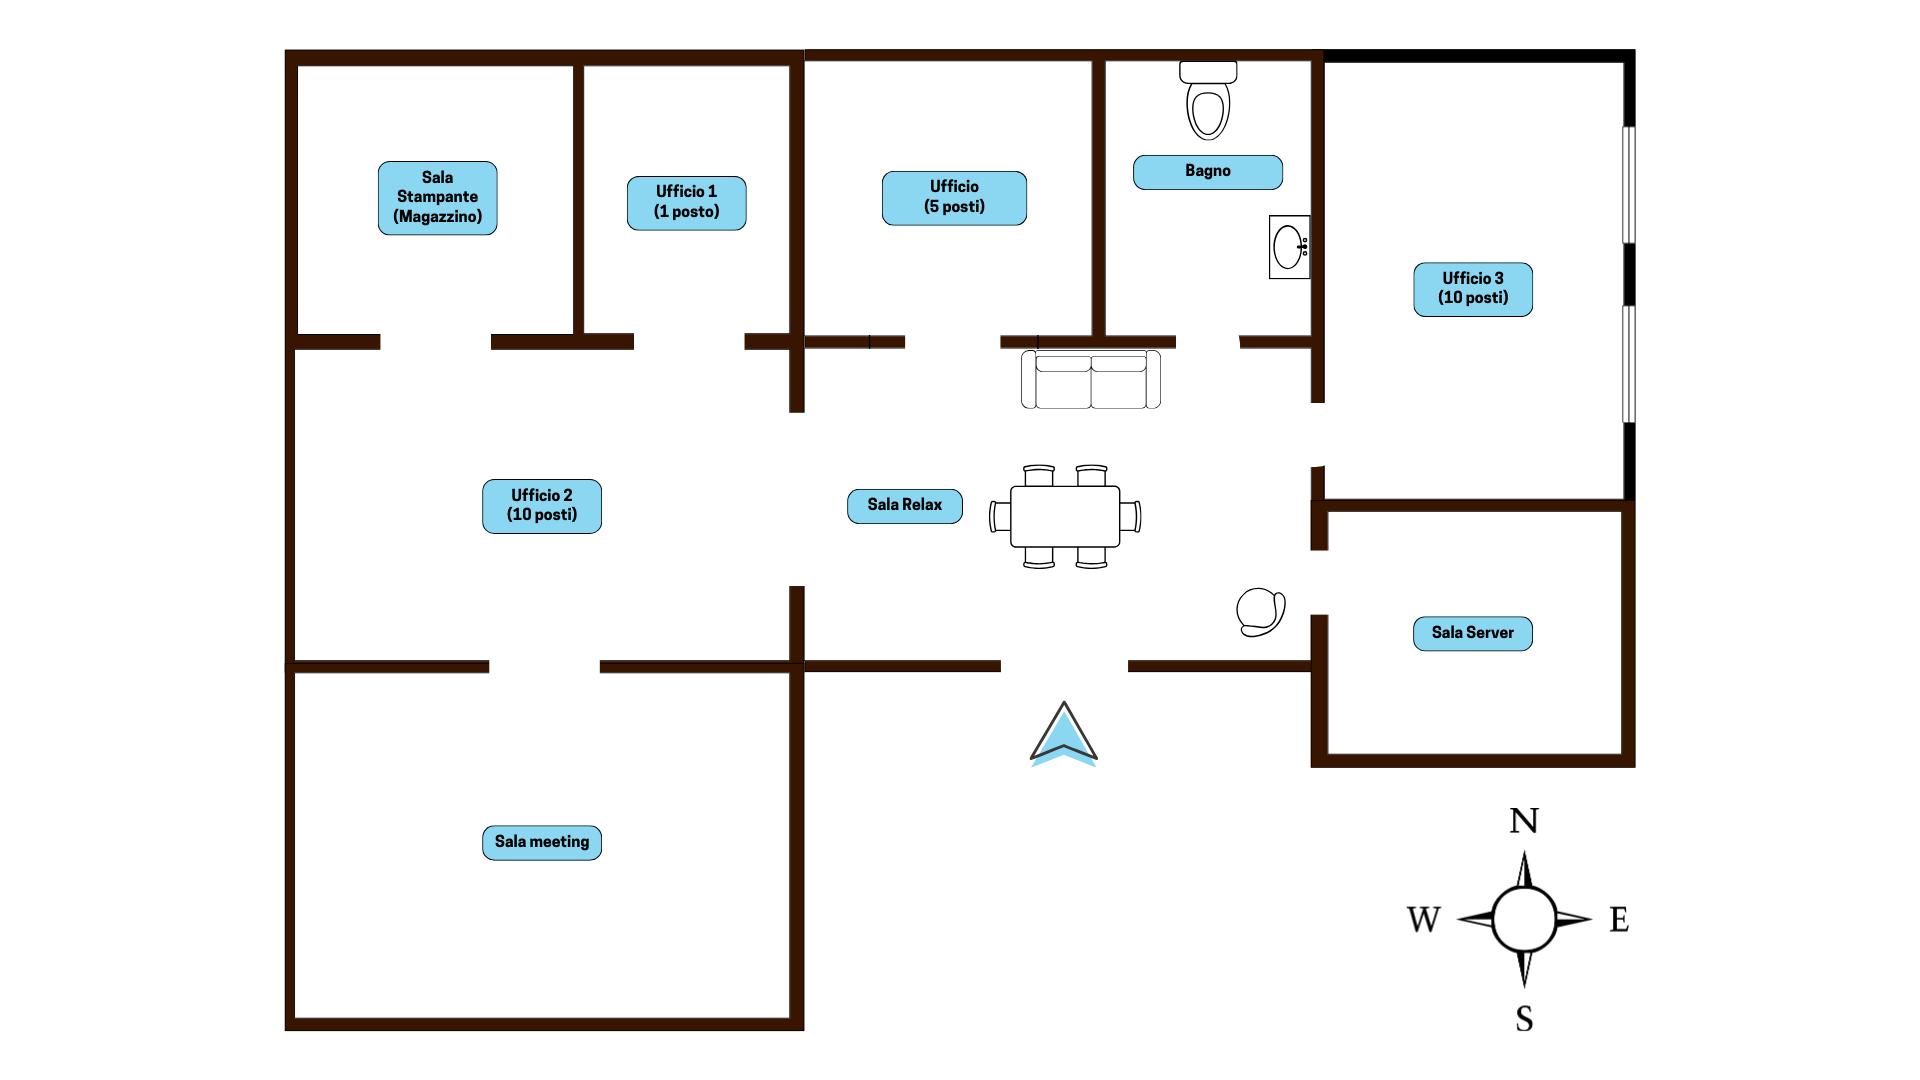
\includegraphics[width=\textwidth]{assets/Floor Plan Ufficio.png}
\captionof{figure}{Planimetria dell'ufficio}\label{fig:floorplan}
\end{center}

Come possiamo vedere dalla immagine \ref{fig:floorplan} l'ufficio è composto da 8 ambienti distinti, ognuno con un utilizzo specifico. Questa suddivisione ci permetterà di progettare una rete che soddisfi le esigenze di ciascun ambiente, garantendo prestazioni ottimali e sicurezza.


\section{Divisione della Rete Interna e Partizione Wi-Fi}
La rete interna sarà suddivisa in più VLAN (Virtual Local Area Network) per isolare i diversi ambienti:

\begin{itemize}
    \item \textbf{VLAN 10}: Uffici principali (Ufficio 2, Ufficio 3, Ufficio 6)
    \item \textbf{VLAN 20}: Uffici speciali (Ufficio 1, Ufficio 7, Ufficio 8)
    \item \textbf{VLAN 30}: Uffici di servizio (Ufficio 4, Ufficio 5)
\end{itemize}

La rete Wi-Fi sarà partizionata in due reti principali:
\begin{itemize}
    \item \textbf{Wi-Fi per i dipendenti}: con accesso a risorse aziendali interne.
    \item \textbf{Wi-Fi per ospiti}: accesso limitato a Internet per maggiore sicurezza.
\end{itemize}

\section{Scelta dei Dispositivi}

\subsection{Dispositivi per connessione LAN Cablata}
I seguenti dispositivi saranno utilizzati dalla connessione LAN cablata:

\begin{table}[H]
    \centering
    \begin{tabular}{>{\bfseries}m{4cm}|m{10cm}}
        \toprule
        \rowcolor{lightblue}
        \textbf{Dispositivo} & \textbf{Ragione di utilizzo} \\
        \midrule
        Server & Garantire velocità di trasferimento dati stabili e rapide, necessarie per applicazioni aziendali critiche \\
        \midrule
        Stampanti & Evitare ritardi di stampa dovuti a possibili interferenze o limiti di connessione wireless \\
        \midrule
        PC degli uffici principali & Garantire velocità di rete massima per attività lavorative intensive e ridurre la congestione della rete Wi-Fi \\
        \bottomrule
    \end{tabular}
    \caption{Dispositivi con connessione LAN cablata e ragione di utilizzo}
    \end{table}
La scelta della connessione cablata è motivata dalla necessità di fornire alte prestazioni e affidabilità, soprattutto per dispositivi che richiedono un traffico dati costante e sicuro.

\subsection {Dispositivi per connessione Wi-Fi}

I seguenti dispositivi saranno preferiti per una connessione Wi-Fi:

\begin{itemize}
    \item \textbf{Smartphone e Tablet}: per la mobilità all'interno dell'ufficio.
    \item \textbf{Laptop}: per la flessibilità di spostamento tra le diverse aree.
    \item \textbf{Dispositivi IoT}: per la connettività senza fili di dispositivi intelligenti.
\end{itemize}


\section{Schema di Rete}

La rete aziendale è progettata per garantire connessioni sicure e ad alte prestazioni. Il \textbf{router} è responsabile della connessione del network aziendale con l'esterno (Internet). Successivamente, il traffico passa attraverso un \textbf{firewall}, che garantisce la sicurezza della rete, filtrando e monitorando i dati in entrata e in uscita. Il firewall è collegato ad uno \textbf{switch principale (core switch)}, che funge da nodo centrale per le connessioni interne.

Dal \textbf{core switch} partono le connessioni verso un \textbf{server}, utilizzato per la gestione dei dati aziendali, e verso due \textbf{switch degli uffici}, che distribuiscono la connettività ai dispositivi delle varie stanze. Gli switch degli uffici sono collegati a tre \textbf{Access Point Wi-Fi} localizzati nei due uffici più grandi e nella sala relax per garantire una copertura wireless efficiente. Inoltre, ogni switch è collegato direttamente ai \textbf{PC fissi} degli uffici tramite \textbf{cavi Ethernet}, per assicurare velocità di connessione elevate e stabili. Questa configurazione garantisce un'architettura di rete bilanciata e sicura, in grado di gestire sia le connessioni cablate che wireless con affidabilità.


\begin{center}
    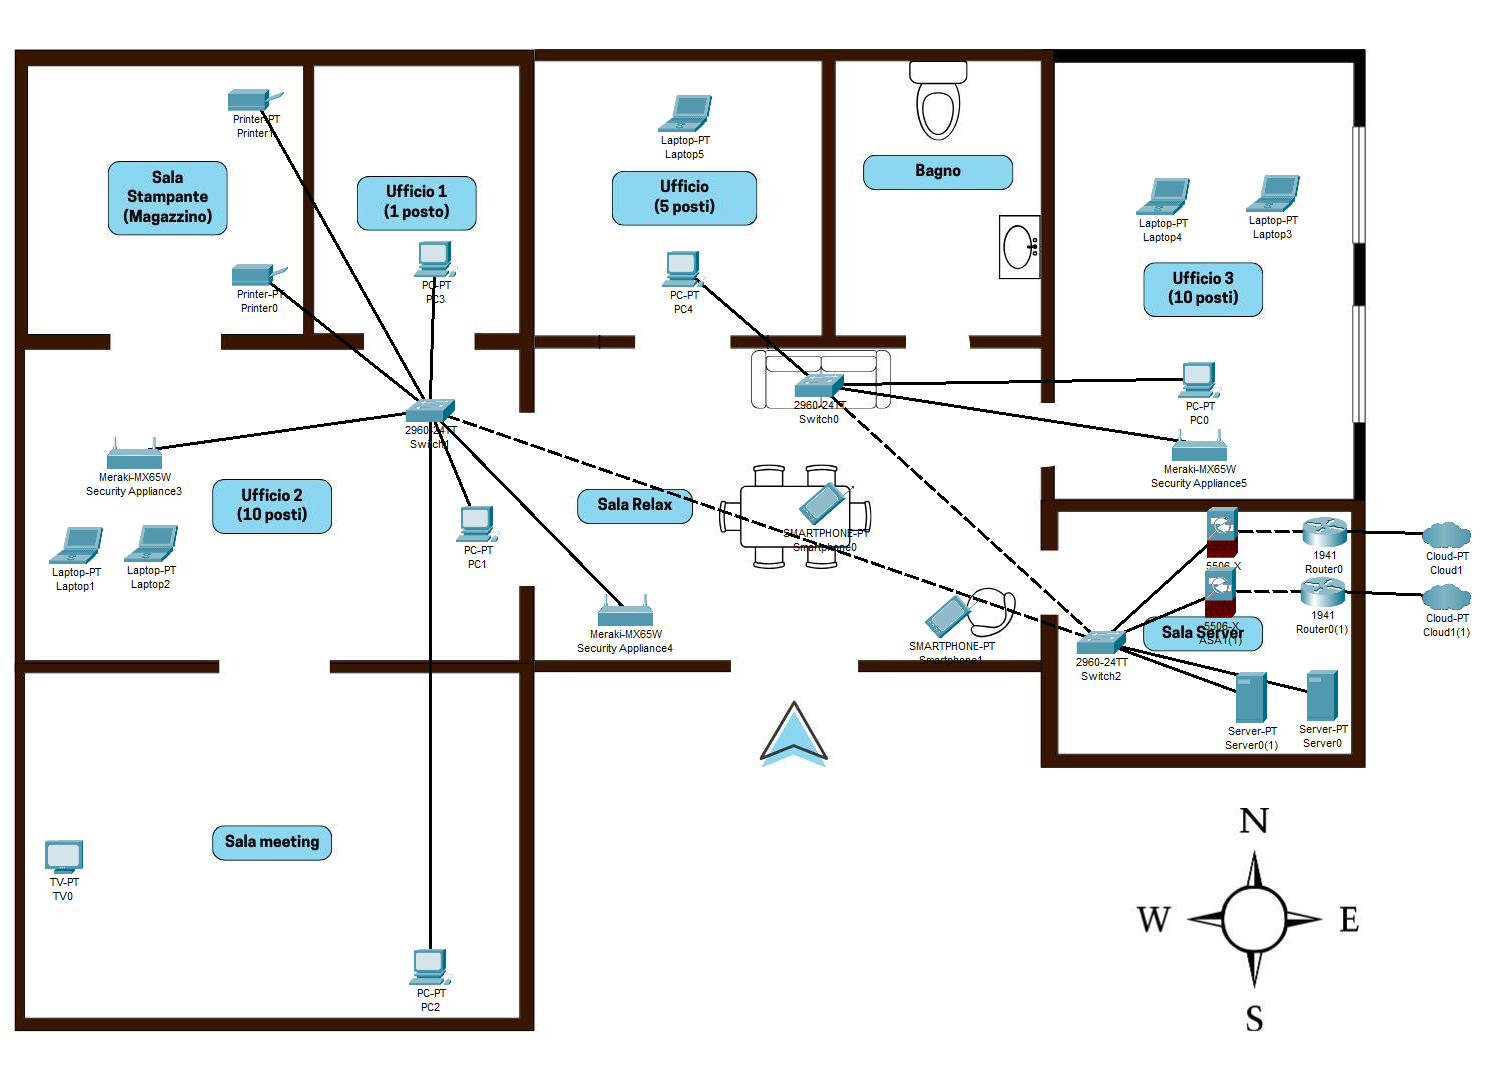
\includegraphics[width=0.8\textwidth]{assets/FloorPlanConDevice.png}
    \captionof{figure}{Schema della rete proposta}
    \end{center}

\subsection{Componenti Hardware della Rete}
La rete è composta dai seguenti dispositivi:

\begin{itemize}
    \item \textbf{Router}: gestione del traffico in entrata e uscita.
    \item \textbf{Switch}: collegamento tra i vari dispositivi interni alla LAN.
    \item \textbf{Firewall}: protezione da minacce esterne e controllo del traffico.
    \item \textbf{Server}: per la gestione delle risorse aziendali.
    \item \textbf{Access Point (AP)}: per la copertura Wi-Fi nell'intero ufficio.
    \item \textbf{Client}: i dispositivi degli utenti finali (computer, stampanti, ecc.).
\end{itemize}


\section{Dispositivi perla sala Conferenze}

Per allestire una sala conferenze funzionale ed efficiente, è necessario selezionare hardware di qualità che garantisca un'ottima esperienza audio e video per le video conferenze e le presentazioni. Di seguito, presentiamo alcuni esempi di hardware essenziali:

\begin{itemize}
    \item \textbf{Logitech Rally Plus}: Un sistema di videoconferenza all-in-one che include una videocamera 4K PTZ, due speaker e microfoni con cancellazione del rumore. Questo sistema è particolarmente adatto per sale di medie e grandi dimensioni, garantendo un'alta qualità audio e video.
    \begin{figure}[H]
        \centering
        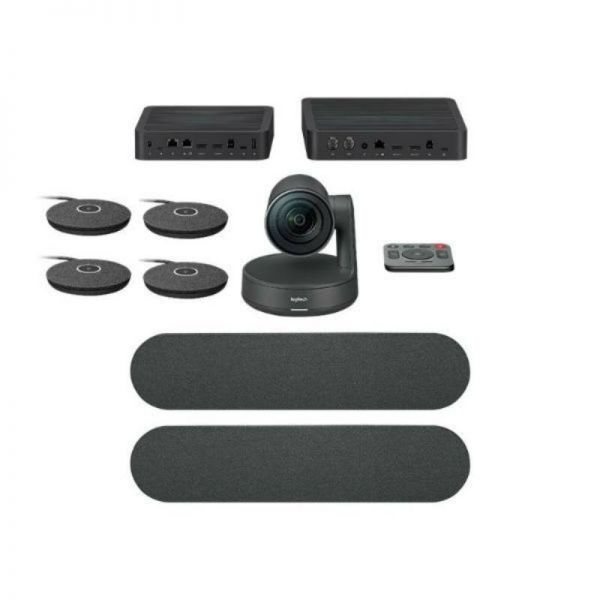
\includegraphics[width=0.2\textwidth]{assets/logitech_rally_plus.jpg}
        \caption{Logitech Rally Plus}
    \end{figure}

    \item \textbf{Jabra Speak 750}: Un altoparlante portatile con funzionalità Bluetooth e USB, ideale per migliorare la qualità audio delle conferenze in stanze di piccole o medie dimensioni. Grazie alla sua compatibilità con diverse piattaforme, come Zoom e Microsoft Teams, è perfetto per riunioni rapide.
    \begin{figure}[H]
        \centering
        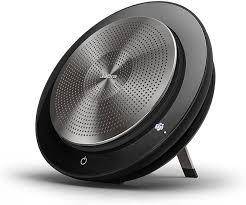
\includegraphics[width=0.2\textwidth]{assets/jabra_speak_750.jpg}
        \caption{Jabra Speak 750}
    \end{figure}

    \item \textbf{BenQ InstaShow}: Un sistema wireless per presentazioni che permette di collegare facilmente computer e dispositivi mobili allo schermo della sala conferenze senza bisogno di cavi. È perfetto per riunioni collaborative e interattive.
    \begin{figure}[H]
        \centering
        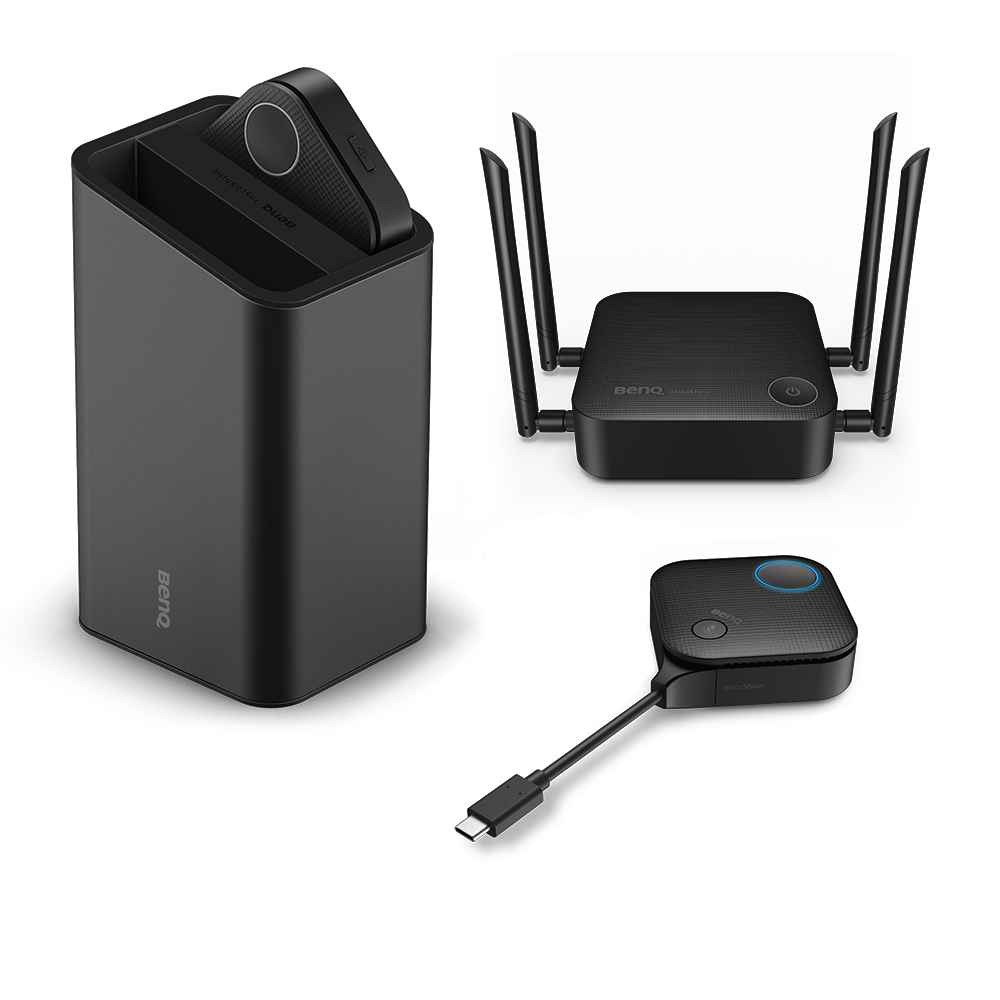
\includegraphics[width=0.2\textwidth]{assets/benq_instashow.png}
        \caption{BenQ InstaShow}
    \end{figure}

    \item \textbf{Samsung Flip 2}: Un display interattivo touch da 65 pollici che permette di prendere appunti e condividere idee in tempo reale durante le riunioni. La sua versatilità e la facilità di integrazione con altri dispositivi lo rendono uno strumento essenziale per sale conferenze moderne.
    \begin{figure}[H]
        \centering
        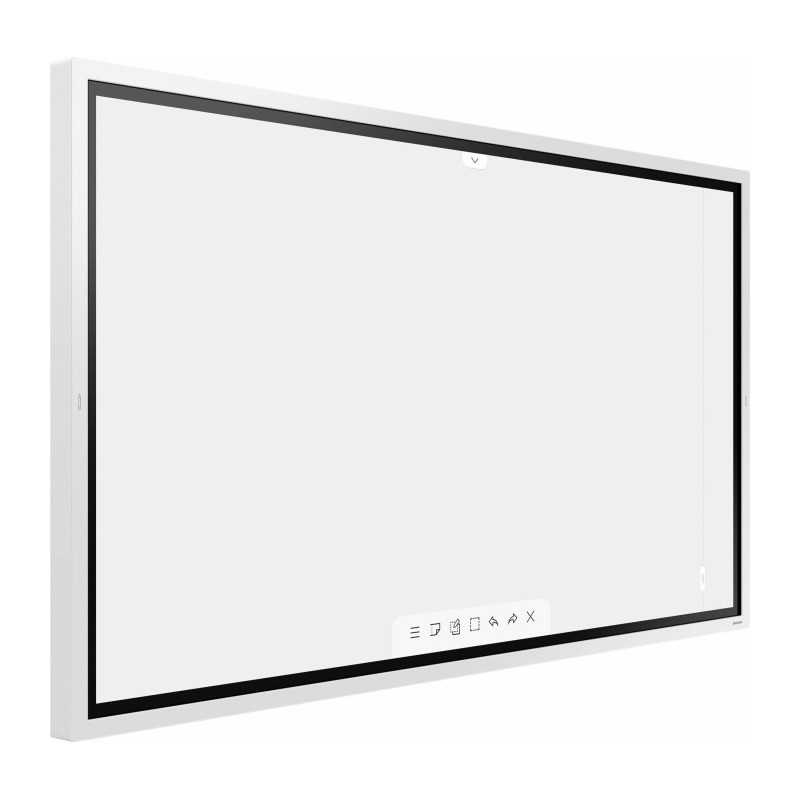
\includegraphics[width=0.2\textwidth]{assets/samsung_flip_2.jpg}
        \caption{Samsung Flip 2}
    \end{figure}
\end{itemize}


Questi dispositivi combinano efficienza, alta qualità e facilità d'uso, rendendoli ideali per creare una sala conferenze moderna e performante.



\section{Conclusioni}
Il progetto di rete per il nuovo ufficio è stato progettato per garantire prestazioni elevate, sicurezza e scalabilità per supportare le esigenze aziendali attuali e future. La scelta di una connessione FTTH, la suddivisione in VLAN e la partizione Wi-Fi consentiranno di ottimizzare le risorse e garantire un'esperienza di rete ottimale per tutti gli utenti. L'uso di dispositivi di qualità per la sala conferenze garantirà un'esperienza audio e video di alto livello per le videoconferenze e le presentazioni. Infine, la ridondanza della connessione Internet e la scelta di operatori affidabili garantiranno la continuità del servizio in caso di guasti o interruzioni. Con queste soluzioni, l'azienda potrà godere di una rete efficiente, sicura e pronta per il futuro.

\end{document}
